%
% diku datanet ACM
%
\documentclass[a4paper,danish]{dnacm} % V0.1
\usepackage{bera}% optional: just to have a nice mono-spaced font
\usepackage{listings}
\usepackage{xcolor}
\usepackage{graphicx}

\colorlet{punct}{red!60!black}
\definecolor{background}{HTML}{EEEEEE}
\definecolor{delim}{RGB}{20,105,176}
\colorlet{numb}{magenta!60!black}
\acmVolume{}
\acmNumber{}
\acmYear{2015}
\acmMonth{}
\acmArticleNum{}
\acmdoi{1}
\setlength\parindent{0pt}
\lstdefinelanguage{json}{
    basicstyle=\ttfamily\small,
    showstringspaces=false,
    breaklines=true,
    frame=lines,
    backgroundcolor=\color{background},
    literate=
     *{0}{{{\color{numb}0}}}{1}
      {1}{{{\color{numb}1}}}{1}
      {2}{{{\color{numb}2}}}{1}
      {3}{{{\color{numb}3}}}{1}
      {4}{{{\color{numb}4}}}{1}
      {5}{{{\color{numb}5}}}{1}
      {6}{{{\color{numb}6}}}{1}
      {7}{{{\color{numb}7}}}{1}
      {8}{{{\color{numb}8}}}{1}
      {9}{{{\color{numb}9}}}{1}
      {:}{{{\color{punct}{:}}}}{1}
      {,}{{{\color{punct}{,}}}}{1}
      {\{}{{{\color{delim}{\{}}}}{1}
      {\}}{{{\color{delim}{\}}}}}{1}
      {[}{{{\color{delim}{[}}}}{1}
      {]}{{{\color{delim}{]}}}}{1},
}


\begin{document}

\title{Assignment 4 \\ RESTful Web Service \\ Datanet 2015} % title

\author{Christian Hohlmann Enevoldsen
\affil{University of Copenhagen}
}

\terms{Programming, Experimentation, API, REST}

\keywords{HTTP, SERVER, CRUD}

\maketitle

\begin{abstract}
In the following a brief introduction to RESTful web services will be given together with a description of a RESTful TODO web server. The design choices, the frameworks used in the service and the basics of how to use it will be covered.
Afterwards the limitations of the web service is outlined and
finally the tests done in this case will be reflected upon. 
\end{abstract}

\section{Introduction}
Most applications deal with data in one form or another. In order to access this data the application needs an interface. There are many different kinds of interfaces like SOAP and REST. This case is going to focus on a RESTful web service. REST (Representational State Transfer) is a specification of remote calls exposed to API consumers. 

In the following sections I am going to describe the implementation of a RESTful TODO web service.

\section{Design}

The following modules/frameworks is used in the Server

\begin{itemize}
\item{\textbf{Node.js}: Non-blocking I/O platform for building the server. }
\item{\textbf{Express}: Used for creating routes and the HTTP Server}
\item{\textbf{Mongoose}: ODM - object data mapping. }
\end{itemize} 

The todo REST server is written in Node.js, and the todo items is stored in MongoDB.
Express is used to ease up routing and server creation. \\

The routes are:

\begin{itemize} 
\item{ \textbf{/} - for the static index file}
\item{ \textbf{/todo} - endpoint for the todo resources.}
\end{itemize} 

Mongoose is an ODM and it is used to connect to the Mongo Database. With Mongoose comes Schemas. Schemas helps define the object data mapping, and eases up the CRUD. There's only one schema defined in the todo server. The todo Schema has the three properties: id, completed and text.

The id is however not an Integer in this case since MongoDB is designed to use Object ID's instead.

The routes can now easily use the built in functions for CRUD operations on the todo Schema, and safely ignore any kind of database communication since that's covered in Mongoose.

\subsection{Using the API}

\textbf{Creating TODO items}

To create a new TODO item a POST request is issued with the following details\\

\begin{lstlisting}[language=json,firstnumber=1]
POST /todo/ HTTP/1.1
Host: localhost:3000
content-type: application/json
Content-Length: 33

{
  "todo" {
    "text": "value"
  }
}
\end{lstlisting}


You can optionally set the completed property. Defaults to false

The response on success is the newly created TODO

\begin{lstlisting}[language=json,firstnumber=1]
HTTP/1.1 201 Created
Content-Type: application/json;
Content-Length: 82
Connection: keep-alive

{
  "todo": {
    "text": "hello world",
    "_id": "556f32f03d8f37d8180ab58e", 
    "completed": false
  }
}

\end{lstlisting}

\textbf{Getting TODO items}

To get all todo items a GET request is issued with following details:

\begin{lstlisting}[language=json,firstnumber=1]
GET /todo/ HTTP/1.1
Host: localhost:3000
Content-type: application/json
\end{lstlisting}

On success the response will be:

\begin{lstlisting}[language=json,firstnumber=1]
HTTP/1.1 200 OK
Content-Type: application/json
Content-Length: 234

{
  "todos": [
    {
      "_id": "556f32f03d8f37d8180ab58e", 
      "text": "hello world", 
      "completed":false
    },
    ...
  ]
}
\end{lstlisting}

To get a specific todo item a GET request is issued with following details:

\begin{lstlisting}[language=json,firstnumber=1]
GET /todo/556f32f03d8f37d8180ab58e HTTP/1.1
Host: localhost:3000
Content-type: application/json
\end{lstlisting}

On success the response will be:

\begin{lstlisting}[language=json,firstnumber=1]
HTTP/1.1 200 OK
Content-Type: application/json
Content-Length: 82

{
  "todo": {
      "_id": "556f32f03d8f37d8180ab58e", 
      "text": "hello world", 
      "completed":false
    }
}
\end{lstlisting}

\textbf{Updating a TODO item}\\

To update a TODO item a PUT request is issued with the following details

\begin{lstlisting}[language=json,firstnumber=1]
PUT /todo/556aeb081eba49a108beffa3 HTTP/1.1
Host: localhost:3000
content-type: application/json
Content-Length: 28

{
  "todo": {
      "completed": true
    }
}
\end{lstlisting}

On success you get the following response

\begin{lstlisting}[language=json,firstnumber=1]
HTTP/1.1 204 No Content
\end{lstlisting}

The content-length is omitted, since newer RFC specs suggests that.


\textbf{Deleting a TODO item}\\

To delete a TODO item a DELETE request is issued with the following details

\begin{lstlisting}[language=json,firstnumber=1]
DELETE /todo/556aeb081eba49a108beffa3 HTTP/1.1
Host: localhost:3000
content-type: application/json

\end{lstlisting}

On success you get the following response

\begin{lstlisting}[language=json,firstnumber=1]
HTTP/1.1 204 No Content
\end{lstlisting}


\textbf{Errors}

If a required property is omitted you can expect the following error response

\begin{lstlisting}[language=json,firstnumber=1]
HTTP/1.1 422 Unprocessable Entity
Content-Length: 46
Content-Type: application/json

{
  "error": {
    "message": "Property todo requried"
  }
}
\end{lstlisting}

For bad syntax expect the following response

\begin{lstlisting}[language=json,firstnumber=1]
HTTP/1.1 400 Bad Requst
Content-Length: 46
Content-Type: application/json

{
  "error": {
    "message": "Unexpected end of input"
  }
}
\end{lstlisting}

For bad URI's you get a 404

\begin{lstlisting}[language=json,firstnumber=1]
HTTP/1.1 404 Bad Request
Content-Length: 76
Content-Type: application/json

{
  "error": {
    "message": "The requested todo item does not exist"
  }
}
\end{lstlisting}


\section{Limitations}

Even though the service only does some trivial logic and the code base is very small there are some major limitations and some minor, which may be features rather than limitations. 

\subsection{Limits}

It is not possible to limit the number of TODO items returned from a request, so you might get a ton of items in response. 

\subsection{Authentication}

As of now no authentication is required when using the API. This means that the server is vulnerable to attacks and misuse. An attacker can easily delete all items in the database by simply getting the list of all items and afterwards delete one by one.

\subsection{Filtering and searching}

It is not possible to filter or search for items. For instance; you might only want to list all completed TODO items, however this requires manual data manipulation on the client side right now. Other than that you cannot search for TODO items containing specific phrases. This results in overhead in data transfer that could have been omitted by doing the operations on the server.  

\subsection{Database}

The server relies on MongoDB running locally on the hosting computer. However the configuration can easily be modified to use another database path. Although you might change the database path you cannot use another kind of database without major refactoring.

\section{Tests}

To make sure that the server is stable and everything works as expected a static webpage is used as a client to the server. The client is a simple website that enables a user to create, modify, delete and see TODO items. The client uses the RESTful API behind the scenes. Arguably any errors in the server would be visually reflected to the user. An interactional test is useful to some point, which includes testing expected results and errors. 

Unit tests is written to make sure that everything is indeed working as expected. Although the interactional website is a great way to test the server, it could easily be discarded in favour of unit tests. 

The unit tests uses a module called Supertest, which other than being able to do unit tests, is useful for testing asynchronous code. The appendix contains a screenshot of the test results. 

\newpage

\appendix

\section{Test}

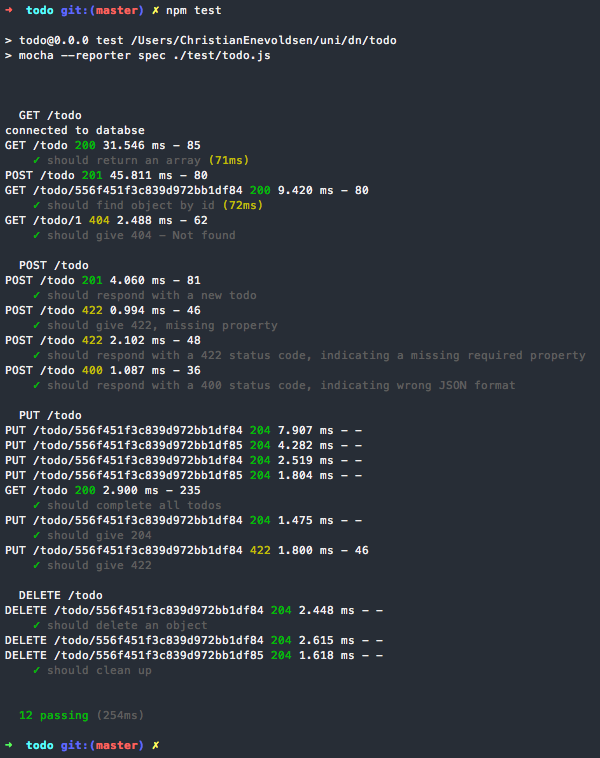
\includegraphics[scale=0.4]{tests.png}

\end{document}
% End of dnacm.tex (April 2015)